\chapter{Methodology}
\label{chap:2}
\ChapterPageStuff{2}

\section{Preamble}\label{sec:ch2_preamble}
 The literature in \Cref{chap:1} is used for the method to create a logging mechanism that can capture user-based activity logs to improve software maintenance by analysing the obtained logs. The development of the solution for the identified problem in \Cref{sec:ch1_problemStatement} will be specifically made for a Web-based application.\par Web-based applications are one the most widely used software implementations that can benefit from a system utilisation analysis using user-based event logs. These software systems have many different designs, for this study Web-applications that require the user to be logged in to an active session in the software system will be used as in \Cref{fig:ch2_webSystemBasic}.

 \begin{figure}[!htb]
	\centering % cent the figure
	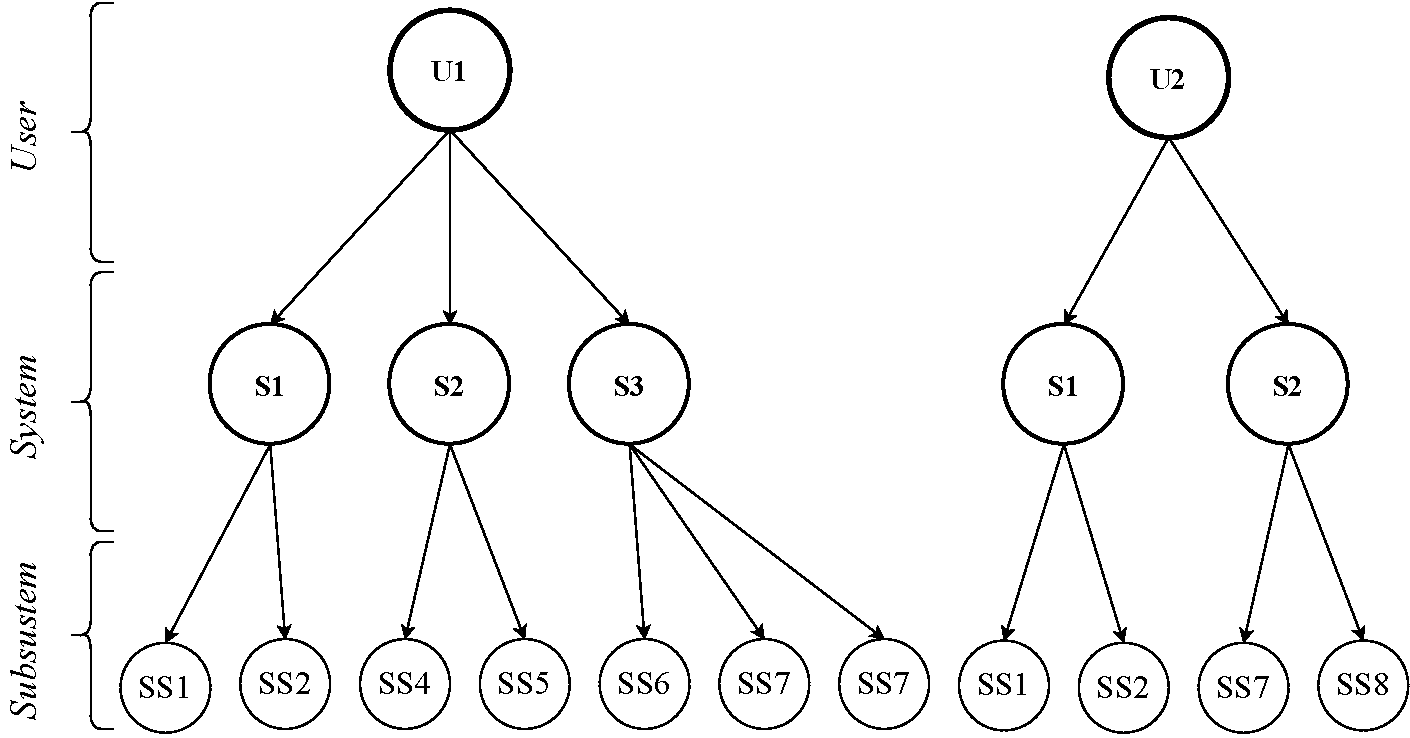
\includegraphics[width=0.95\textwidth]{img/Chapter2/systemOverview/systemOverview.pdf}
	\caption[Basic design of a software system]
	{\textit{Basic design of a software system}}\label{fig:ch2_webSystemBasic}
\end{figure}
 
 In \Cref{fig:ch2_webSystemBasic} is the basic design of the Web application the users interact with different systems. These systems can be different pages or sections of the website and can be further divided into subsystems. \par In \Cref{sec:ch2_loggingMechanism} the methodology to create a logging mechanism to capture user-generated events is discussed for web-based applications. The different functional requirements and interfaces are discussed in this section \cite{Anish2015}.\par In \Cref{ch2:sec_system_utilisation_analysis} the methodology is discussed to analyse these obtained logs to improve software maintenance by using various tools visualisation tools or creating them based on the available log attributes.

 \clearpage

\section{Development of solution}\label{sec:ch2_developementOfSolution}
In \Cref{sec:ch1_objectives} the objectives of the study are split into two main parts that need to be implemented to solve the identified problem. The logging mechanism and log analysis of the obtained logs. A basic system design can be made for the logging mechanism. In \Cref{fig:ch2_systemDesign} is the design for the logging mechanism to capture the user-based event logs.

\begin{figure}[!htb]
	\centering % cent the figure
	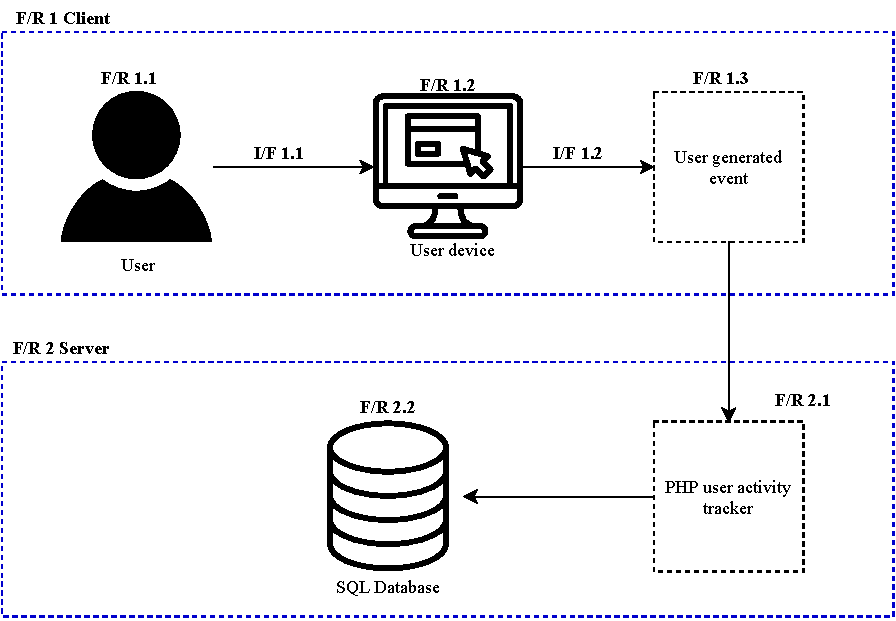
\includegraphics[width=0.95\textwidth]{Chapter2/SystemA_Architecture_Diagram/SystemA_Architecture_Diagram.pdf}
	\caption[Logging mechanism basic system design]
	{\textit{Logging mechanism basic system design}}\label{fig:ch2_systemDesign}
\end{figure}

In \Cref{fig:ch2_systemDesign} is the basic system design of the logging mechanism. This design provides a high-level overview of the interaction the user has with the software system to create a user-based event log. The two sides of the design in \Cref{fig:ch2_systemDesign}:

\begin{itemize}
	\item \textbf{Client} side which involves the user, the device the user uses to access the website and the user-generated event. The user interacts with the website, this creates a user event that can be captured. 
	\item \textbf{Server} side which has the rest of user activity logging software that consists of multiple or a single logging point. The user activity logger interacts with a structured database to store the captured log created from all the captured log attributes.
\end{itemize}

The two main parts are to create a logging mechanism to capture the user-based activity logs and log analysis to prioritise software maintenance of the study objectives in \Cref{sec:ch1_objectives} is illustrated in \Cref{fig:ch2_developmentOfSolution}.

\clearpage

\begin{figure}[!htb]
	\centering % cent the figure
	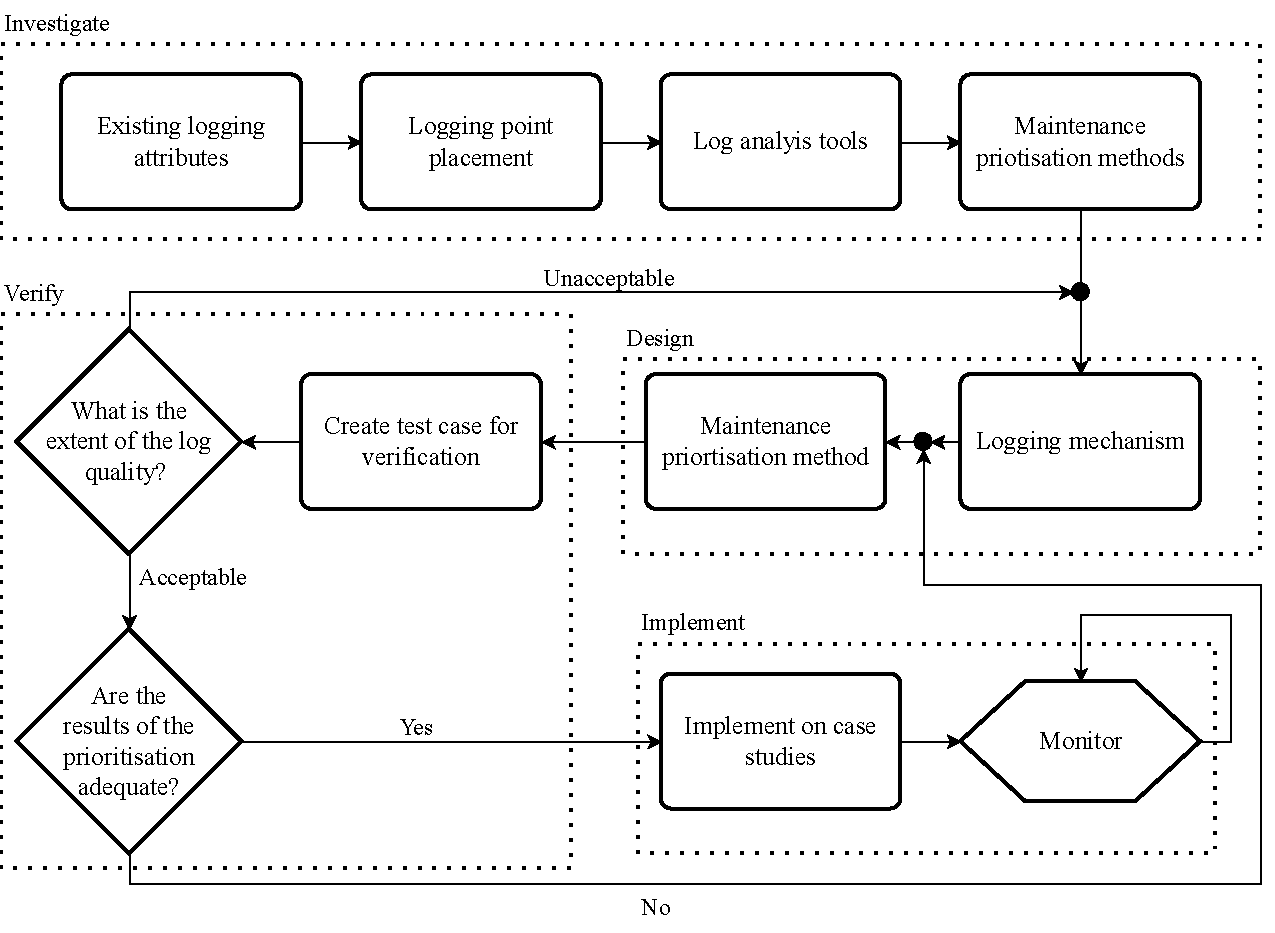
\includegraphics[width=0.95\textwidth]{img/Chapter2/developmentOfSolution/developementOfSolution.pdf}
	\caption[Development of solution overview]
	{\textit{Development of solution overview}}\label{fig:ch2_developmentOfSolution}
\end{figure}

\Cref{fig:ch2_developmentOfSolution} is a high-level overview of the development of the solution. Each of the main development steps is to create the logging mechanism to do a log analysis for software maintenance prioritising. These main development steps will be further discussed in detail and in \Cref{tbl:ch2_developmenetRequirements} is the summary of each of the main development functional requirements.

\setcounter{phase}{0}
\begin{table}[!htb]
	\centering
	\caption[Development of solution functional requirements]
	{\textit{Development of solution functional requirements}}
	\label{tbl:ch2_developmenetRequirements}
	\begin{tabularx}{\textwidth}{|l|l|X|}
		\hline \textbf{Requirement ID} & \textbf{Name} & \textbf{Description} \\
		\hline \phase{fr:logAttributes} & Identify log attributes & \RaggedRight The log attributes need to be identified as what is needed to complete the log analysis for software maintenance prioritisation. The log attributes form the characteristics of the obtained event which for this study focuses on user-based events. \\
		\hline \phase{fr:loggingPoints} & Logging point creation & \RaggedRight Log points capture the desired log attributes when the user-based event is taking place. In \Cref{sec:ch1_loggignPoints} logging points should be strategically placed in the software system to capture the event logs. This stage of the development includes identifying where the log points should be placed, log creation and database interactions.\\
		\hline \phase{fr:logAnalysis} & \RaggedRight Create or use log analysis tools & Make use of suitable third-party tools or create software to do log analysis on the stored event logs. \\
		\hline \phase{fr:maintenancePrioritising} & \RaggedRight Maintenance prioritising & Create a maintenance prioritising report based on the log analysis for software maintenance using the log analysis tool. The report aims to visualise the system utilisation of certain parts of the system and determine maintenance prioritisation.\\
		\hline
	\end{tabularx}
\end{table}

The functional requirements (\textbf{F/R}) in \Cref{tbl:ch2_developmenetRequirements} are used to identify each requirement for the development of a solution that can be later verified. Sub-requirements will use the same labelling. 

\section{Logging mechanism}\label{sec:ch2_loggingMechanism}
The logging mechanism system design will be defined in this section. This is to create a generic method of how to create a suitable logging mechanism to capture specific user-based event logs. This also defines any other sub-functional requirements to identify the log attributes (\ref{fr:logAttributes}) and logging point creation (\ref{fr:loggingPoints}).

\subsection{Log attributes requirements}\label{sec:ch2_logAttributesRequirements}
The log attributes functional requirement (\ref{fr:logAttributes}) focuses on the possible events that the user has been involved with when interacting with the software system. In \Cref{tbl:ch2_loggingAttributesFunctionalRequirements} are the functional requirements of \ref{fr:logAttributes}.

\setcounter{phase}{1}
\begin{table}[!htb]
	\centering
	\caption[Log attributes functional requirements (\ref{fr:logAttributes})]
	{\textit{Log attributes functional requirements (\ref{fr:logAttributes})}}
	\label{tbl:ch2_loggingAttributesFunctionalRequirements}
	\begin{tabularx}{\textwidth}{|l|l|X|}
		\hline \textbf{Requirement ID} & \textbf{Name} & \textbf{Description} \\
		\hline \subphase{fr:userEventReq} & \RaggedRight User-based event log characteristics & \RaggedRight This functional requirement defines the characteristics of what software system events can be classified as a user-based event. \\
		\hline \subphase{fr:userActReq} & \RaggedRight User activity types & \RaggedRight User activity types further expand on what event types are valid of \ref{fr:userEventReq}. This is also the first categorisation of the obtained logs.\\
		\hline \subphase{fr:subLogAttributes} & \RaggedRight Log attributes & \RaggedRight The log attributes are the obtained data that describes a user-based event log. This is the primary data that will be stored in a structured database.\\
		\hline
	\end{tabularx}
\end{table}

\Cref{tbl:ch2_loggingAttributesFunctionalRequirements} is the first functional requirement for the development of a solution that needs to be defined. It is important to define and create the event log characteristics for a user-based event log. The rest of the logging mechanism depends on what needs to be logged as discussed in \Cref{sec:ch1_eventLogging} about the importance of what events need to log. 

\subsubsection{User-based event log characteristics}\label{sec:ch2_requirementsOfUAT}
The user is the initiator of the logging mechanism. Each action or event they trigger by interacting with the user interface on their device can be a potential user-generated event. In \Cref{tbl:ch2_requirementsForUserActivtyEvent} is the sub-requirements for the user that the event log should fulfil to be classified as a user-based activity log.

\clearpage

\setcounter{phase}{1}
\setcounter{subphase}{1}
\begin{table}[!htb]
	\centering
	\caption[Requirements for an event to be a user-based activity]
	{\textit{Requirements for an event to be a user-based activity}}
	\label{tbl:ch2_requirementsForUserActivtyEvent}
	\begin{tabularx}{\textwidth}{|l|X|}
		\hline \textbf{Requirement ID} & \textbf{Description}\\
		\hline \subsubphase{fr:requirementsUserBased1} & The event has to be triggered by the user interacting with the user interface using their device and not any other events that the system will self-initiate. The user needs to have interacted with the UI directly. This can also be validated by tracking if the user did interact with the UI from the HTML element ids. \\
		\hline \subsubphase{fr:requirementsUserBased2} & The event must consist of different cases ($ca~ \epsilon~CA$ the cases consists of events) which are noteworthy to make the event log identifiable \cite{Slaninova2014}. \\
		\hline \subsubphase{fr:requirementsUserBased3} & For certain types of event logs for \ref{fr:requirementsUserBased2}, the user-generated event should have an origin from which the event took place. \\
		\hline \subsubphase{fr:requirementsUserBased4} & The event log should consist of attributes that expand the identity of the user-based activity. \\
		\hline \subsubphase{fr:requirementsUserBased5} & The event must have the user as the initiator or input for the user-based activity. This will exclude all events triggered by the system as the user did not directly start the event. \\
		\hline \subsubphase{fr:requirementsUserBased6} & Only use the first \textit{HTTP requests}\footnote{A \textbf{HTTP request} is made by a client, to a named host, which is located on a server. The request aims to access a resource on the server. \cite{IBM2021}.} that is sent to the server. \\ 
		\hline
	\end{tabularx}
\end{table}

Every interaction the user has with the user interface of the device to the software system can be seen as an event triggered by the user. Most of these events won't have a meaningful impact as they won't fulfil \ref{fr:requirementsUserBased2} and \ref{fr:requirementsUserBased4} in \Cref{tbl:ch2_requirementsForUserActivtyEvent}.\par For the user activity event to meet the requirement of \ref{fr:requirementsUserBased2} it has to have defined cases that describe the activity type of each event. These activity types form the basic criteria for which events can be parsed which significantly reduces the number of logs that will be obtained. This will ensure that the event logging process will produce quality user-based logs as discussed in \Cref{sec:ch1_loggingQuality}:

\begin{itemize}
	\item A basic structural complexity to simplify log parsing and development of the logging points in the system,
	\item Keep the logging consistent by not deviating from the defined cases, and
	\item Ensure that the event log's other attributes are complete and available to increase the accuracy and trustworthiness of the event logging when further system utilisation analysis needs to be done. 
\end{itemize}

\subsubsection{User activity types}\label{sec:ch2_userActivityTypes}
The user activity types (\ref{fr:userActReq}) categorise different user-based event logs when they are obtained before other log attributes are completely defined. In \Cref{tbl:ch2_userActivityTypes} is the basic user activity types functional requirements.

\clearpage

\stepcounter{subphase}
\begin{table}[!htb]
	\centering
	\caption[User activity types]
	{\textit{User activity types}}
	\label{tbl:ch2_userActivityTypes}
	\begin{tabularx}{\textwidth}{|l|l|X|}
		\hline \textbf{Requirement ID} & \textbf{Activity Type} & \textbf{Description} \\
		\hline \subsubphase{fr:uatType1} & Web page accessed & The user may navigate through different web pages in a session. This is to track when the user initially accessed a certain web page or software system on the page.\\
		\hline \subsubphase{fr:uatType2} & Session changes & This is any user activities excluding \ref{fr:uatType1} that modifies the user's session:
		\begin{itemize}
			\item Logging into a Web application. Both Successful and failed attempted logins. This user-based activity may cause the log attributes that identify the user will be a \texttt{NULL} value as the user's session has not started yet to verify their identity,
			\item Ending their session by logging out or declining to extend their session when it is about to expire,
			\item Modifying any session or other relevant variables that can be used in the utilisation analysis
		\end{itemize}\\
		\hline \subsubphase{fr:uatType3} & General activity & Any events excluding the first two user-based activity types that the user initiates when they interact with the web page. Most of the user activity logs will
		have this event type.\\ 
		\hline
	\end{tabularx}
\end{table}

The general user activity event type (\ref{fr:uatType3}) will the be most common user activity event and be split up into different user activity events. This is determined by the need of what utilisation stage requires to analyse specific user activity events. \par These user activity types can be further expanded with the general activity (\ref{fr:uatType3}) for log analysis purposes. The general activity types will be different for each system based on what the system enables the user to do or what is needed for further system utilisation analysis such as determining if the action the user triggered was to generate a report that they downloaded.

\subsubsection{Log attributes}\label{sec:ch2_logAttributes}
The log attributes (\ref{fr:subLogAttributes}) are the descriptive characteristics of the user-based event logs. The functional requirements for the log attributes are defined in \Cref{tbl:ch2_keyLoggingAttributes}.

\clearpage

\stepcounter{subphase}
\begin{table}[!htb]
	\centering
	\caption[Logging attributes]
	{\textit{Logging attributes}}
	\label{tbl:ch2_keyLoggingAttributes}
	\begin{tabularx}{\textwidth}{|l|l|X|}
		\hline \textbf{Requirement ID} & \textbf{Logging point} & \textbf{Description} \\
		\hline \subsubphase{fr:lpa1} & Identification number & The activity identification is an incremental number of the user-based event that is logged.\\
		\hline \subsubphase{fr:lpa2} & Timestamp & This is the time the user initiated the user-based activity event. This will be the timestamp the log was written into the database as the log will be made before the rest of the intended \textit{HTTP request} is completed. \\
		\hline \subsubphase{fr:lpa3} & Activity type & Each event can be classified into user-based types. This is the user-based activity types in \Cref{tbl:ch2_userActivityTypes}.\\
		\hline \subsubphase{fr:lpa4} & User identification & Each user has a unique identification number that links the event to them if their session has been verified and can be obtained. Will not be available when the user tries to log in to the system as their session has not been set yet. \\
		\hline \subsubphase{fr:lpa5} & Request origin & In web applications, there are always requests sent back to the server which will call the primary function to handle the request. This can be logged as either the file that the request is being sent to or the Web page from which the request came. \\
		\hline \subsubphase{fr:lpa6} & Metadata & The metadata of the event contains request parameters or other relevant request data of the event. This metadata adds more information about the user's activity. Some of the event types may not have metadata added. \\
		\hline \subsubphase{fr:lpa7} & Miscellaneous & These are any non-metadata attributes that can be consistently captured to be used in the utilisation analysis. They expand the characteristics of the obtained user-based log beyond the base attributes. \\ \hline
	\end{tabularx}
\end{table}

The defined logging attributes in \Cref{tbl:ch2_keyLoggingAttributes} are the base attributes that form part of the main structure of the user-based event log. For web-based applications on the client side, only some of these attributes can be obtained as the rest of the attributes can be resolved on the server side. The metadata (\ref{fr:lpa6}) can consist of the request parameters that are obtainable on the server side but any additional captured data can be added and sent to the server.

\clearpage

Each of these log attributes combined creates the base log from which key logging points can be created in the software system to capture the user-based activity logs in \Cref{tbl:ch2_keyLoggingAttributes}. The activity type (\ref{fr:lpa3}) can be assigned during the user-based activity identification phase with a default value and resolved to a new activity type based on metadata or other parameters by:

\begin{itemize}
	\item If it alters any of the session variables that are relevant to the system utilisation analysis,
	\item Access a certain part of the software system that needs all the user-based activities set to a certain type based on the nature of the procedures that need to be executed such as triggering a generation of a report that can be its user-based activity type.
	\item The activity type is also sorted by HTML element tags such as a button or text box.
\end{itemize}

There can be extra parameters captured on the client side such as by the logging point or can either be captured on the server side when the rest of the log's attributes are being obtained. These extra parameters are shown in \Cref{fig:ch2_MetadataJsonExample}.

\begin{lstlisting}[style=json, caption={\textit{Metadata JSON}}, label={fig:ch2_MetadataJsonExample}] 
	{ "RequestTarget" : "/Area4/Controller4/TestFunction",
		"RequestElementID" : "Button4",
		"RequestParameters": {
			"Parameter1": 4,
			"Parameter2": "Hello World!",
			"Parameter3": true
			"Parameter4": 40.404
			"Parameter5": {
				"Parameter6": "Car",
				"Parameter7" 160000.00
			}
		}		
	}
\end{lstlisting}

The metadata in \Cref{fig:ch2_MetadataJsonExample} is the possible extra parameter that can be obtained for the user-base activity log. The metadata will need to store as a JSON string as it can be a complex object that doesn't have a set number of parameters. This complex object can have:

\begin{itemize}
	\item The \texttt{RequestTarget} parameter can be a file path for the Website code from which the page is created or a software system. It also contains the function that is being called by the \textit{HTTP request}.
	\item The \texttt{RequestElementID} is the HTML element id with which the user interacted which caused the user-based activity. This can be used as another validation that the event was caused by the user. Some of the user-based activities can be set to some of these HTML element types by getting the HTML element tag.
	\item The \texttt{RequestParameters} is all the parameters in the \textit{HTTP request} that can be serialised into a JSON string. This can be used to determine what the user tried to do by using this input for the specific function which is used for \ref{fr:requirementsUserBased6} in \Cref{tbl:ch2_requirementsForUserActivtyEvent}.
\end{itemize}

\subsection{Web application architecture}\label{sec:ch2_webApplicationArchitecture}
To determine the user activity types for a Web application, the Web application's architecture will be a factor in the logging mechanism. Web applications consist mostly of HTML, JavaScript and CSS programming languages. The Model-View-Controller (MVC) architecture is mostly used for web-based applications using that programming language \cite{Jailia2016}. The MVC architecture in \Cref{fig:ch2_flowMVC_Architecture} consists of 3 basic parts which are the \cite{Jailia2016}:

\begin{itemize}
	\item \textit{Model:} Is the representation of the records in the database which also interacts with the database through a database access layer or service manipulating the data by using the CRUD operations:
	\begin{itemize}
		\item \textit{create} operation that adds new data,
		\item \textit{read} operation that gets the data from the database,
		\item \textit{update} operation that modifies the existing data,
		\item \textit{delete} operation that removes data.
	\end{itemize}
	\item \textit{Controller:} Is operates both the \textit{View} and \textit{Model} and serves as the connection between the user and the system by controlling the data flow of the \textit{Model} and
	\textit{View}.
	\item \textit{View:} This shows the results of the data contained in the \textit{Model} and enables the user to manipulate the data. The user will only interact with this part of the Web application.
\end{itemize}

\begin{figure}[!htb]
	\centering % cent the figure
	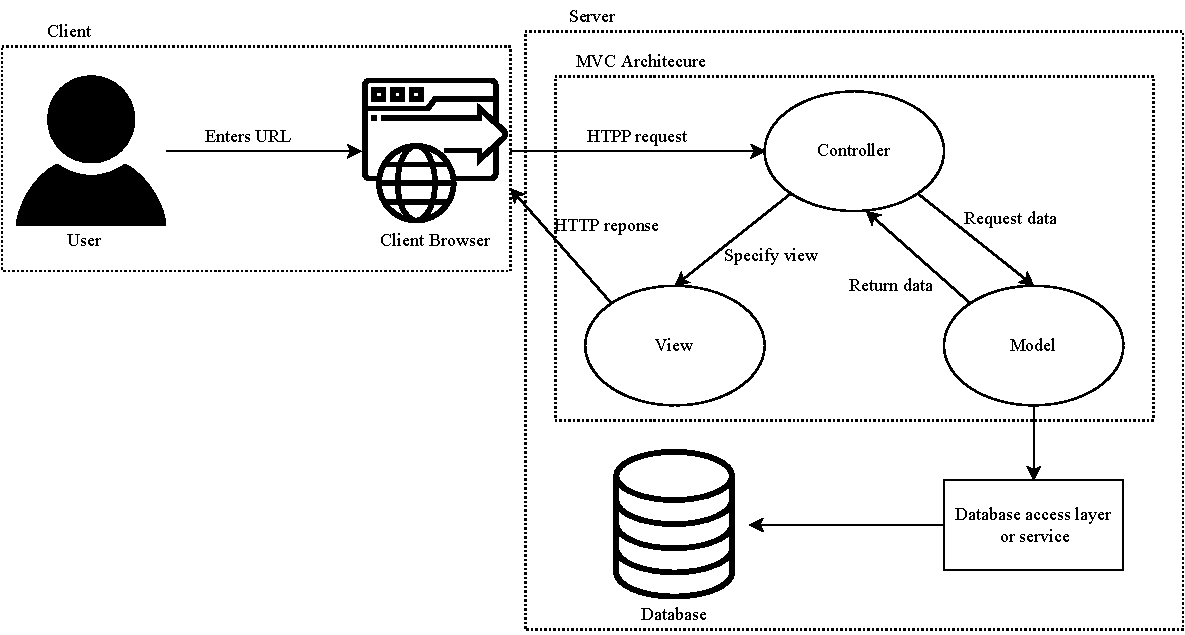
\includegraphics[width=0.9\textwidth]{Chapter2/Flow_MVC_Architecture/Flow_MVC_Architecture.pdf}
	\caption[MVC architecture for most web-based applications]
	{\textit{MVC architecture for most web-based applications \cite{Gu2010}}}\label{fig:ch2_flowMVC_Architecture}
\end{figure}

In \Cref{fig:ch2_flowMVC_Architecture} is the MVC architecture equivalent representation of \Cref{fig:ch2_systemDesign} where the data flow is shown of the MVC architecture. The user interacts with the Web application through their browser which will send a \textit{HTTP requests} to the \textit{Controller} and receive a \textit{HTTP response}\footnote{An \textbf{HTTP response} is made by a server to a client. The response aims to provide the client with the resource it requested, inform the client that the action it requested has been carried out, or else inform the client that an error occurred in processing its request. \cite{IBM2021a}.} from the \textit{View}.The \textit{Controller} will request and return the data to the \textit{Model} which interacts with the database access layer or service to do the \textit{create}, \textit{update} and \textit{delete} operations.\par To classify any interaction between the user (F/R 1) and server (F/R 2) to fulfil the functional requirements of \Cref{tbl:ch2_requirementsForUserActivtyEvent} only the \textit{HTTP request} are used for the logging points in \Cref{sec:ch2_loggingPoints} as it:

\begin{itemize}
	\item Meet the \ref{fr:requirementsUserBased1} and \ref{fr:requirementsUserBased1} as the user will interact with the \textit{View} to modify the data which needs to send back an \textit{HTTP request} to process the data on the \textit{Controller}.
	\item User activity types can be assigned for different scenarios the user triggers when the request is sent. 
	\item Any additional metadata can be sent with the \textit{request header}\footnote{A \textbf{request header} is an HTTP header that can be used in an HTTP request to provide information about the request context so that the server can tailor the response. For example, the Accept-$\ast$ headers indicate the allowed and preferred formats of the response. \cite{Mozilla2022}.} of the \textit{HTTP request}. This will reduce the overhead added by the logging mechanism by not sending additional \textit{HTTP request} each time back to the server when a user-based activity has been identified.
\end{itemize}

\subsection{Logging point requirements}\label{sec:ch2_serverFunctionalRequirements}
The logging point functional requirement (\ref{fr:loggingPoints}) focuses on the creation and strategic placement of the logging points. The log points that obtain the logging attributes must also store the created event log in a structured database. The logging point's sub-functional requirements are defined in \Cref{tbl:ch2_loggingPointsFuntionalRequirements}. 

\stepcounter{phase}
\begin{table}[!htb]
	\centering
	\caption[Logging points functional requirements (\ref{fr:loggingPoints})]
	{\textit{Server functional requirements (\ref{fr:loggingPoints})}}
	\label{tbl:ch2_loggingPointsFuntionalRequirements}
	\begin{tabularx}{\textwidth}{|l|l|X|}
		\hline \textbf{Requirement ID} & \textbf{Name} & \textbf{Description} \\
		\hline \subphase{fr:serverActivityLogger} & Logging point placement & The logging points are used to capture and create the user-based event log that will be stored in a database.\\
		\hline \subphase{fr:serverDatabase} & Storing the user-based activity logs & The event log is stored in a structured database until it is needed for further log analysis.\\
		\hline
	\end{tabularx}
\end{table}

\Cref{tbl:ch2_loggingAttributesFunctionalRequirements} concludes the design requirements for the logging mechanism. The stored logs will be further processed when the log analysis needs to be implemented.

\subsubsection{Logging point placement}\label{sec:ch2_loggingPoints}
In \Cref{sec:ch1_loggignPoints} the logging points should be strategically placed in the software system to capture the log attributes for the user-based activity log. To meet the requirements of \Cref{tbl:ch2_requirementsForUserActivtyEvent} for a user-based activity the logging points should adhere to the logging points functional requirements of \Cref{tbl:ch2_loggingPointRequirement}.

\clearpage

\setcounter{phase}{2}
\setcounter{subphase}{1}
\begin{table}[!htb]
	\centering
	\caption[Logging points requirements]
	{\textit{Logging points requirements}}
	\label{tbl:ch2_loggingPointRequirement}
	\begin{tabularx}{\textwidth}{|l|X|}
		\hline \textbf{Requirement ID} & \textbf{Description} \\
		\hline \subsubphase{fr:lp1} & The logging point should be placed where the user's interaction with the software system will send a \textit{request} back to the server.\\
		\hline \subsubphase{fr:lp2} & Each logging point should consistently capture the user-based activity as the activity is happening. \\
		\hline \subsubphase{fr:lp3} & Logging points should be globally complete to capture the user-based activities in the giving software system without too much modification between each point in the same
		software system. \\
		\hline \subsubphase{fr:lp4} & The logging points should not interfere with the rest of the system's operations, this would be slowing down the system by causing too much overhead in each \textit{request}
		that is being sent. \\
		\hline
	\end{tabularx}
\end{table}

The logging points can either be a single code segment or consist of multiple code segments in a software system that aims to capture user-based actions as they happen. Creating multiple logging points in a software environment will:

\begin{itemize}
	\item Increase complexity of the logging mechanism. Each point can be different from the other as it will need certain operations to capture the log,
	\item The consistency of the logging might differ and increase as the logging points increase in a software system. 
	\item The correctness of the logging will be impacted if the different changes in the logging point if the logging points are unable to consistently capture the user-based activity or extract all the needed attributes to complete the user-based log.
\end{itemize}

Creating a single logging point reduces the complexity and in most cases will improve the consistency and correctness of the user-based logs. In Web applications, a globally defined logging point can be used in a modified \textit{HTTP request} that will form the base template for all or most \textit{HTTP request} used in the software system as in \Cref{sec:ch2_webApplicationArchitecture}.\par The use of a single centralised logging point doesn't guarantee that the logging mechanism will perform more efficiently and accurately than using multiple logging mechanisms. Using a single logging point may have complexity issues when it needs to capture each user-based activity consistently with different cases.

\subsubsection{Storing the user-based activity logs}\label{sec:ch2_databaseStorage}
After the logging point has captured the log attributes and created the event log, the log can be saved in a structured database. The storing of the user-based logs functional requirements (\ref{fr:serverDatabase}) should be defined for structured database interactions.\par The captured parameters of the log attributes may have some sensitive user data that should not be logged. Functions can be excluded or assigned a new user activity type that will need to filter out certain parameters or not log any parameters a all. This will be any functions that include:

\begin{itemize}
	\item Session handling functions that contain passwords or other user information that should not be available for anyone but the user. This could lead to unintentional information disclosure of any personal information in the system utilisation analysis if it is available for anyone who can see and use the user-based activity logs,
	\item Complex parameters such as file upload streams of files that the user tries to upload. This information cannot be broken down to a simple \texttt{JSON} structure as in \Cref{fig:ch2_MetadataJsonExample}, other metadata such as the file size, name and type can rather be logged. This can also be defined as a separate user-based activity event type by detecting these complex parameters.
\end{itemize}

In \Cref{tbl:ch2_SQLLoggingTable} is the data type of the parameters and the functional requirements that it needs will need to fulfil of \Cref{tbl:ch2_keyLoggingAttributes}.

\stepcounter{subphase}
\begin{table}[!htb]
	\centering
	\caption[Log attributes for database storing of the event logs]
	{\textit{Log attributes for database storing of the event logs}}
	\label{tbl:ch2_SQLLoggingTable}
	\begin{tabularx}{\textwidth}{|X|X|X|X|}
		\hline \textbf{Requirement ID} & \textbf{Column Name} & \textbf{Data Type} & \RaggedRight \textbf{Log attribute requirement} \\
		\hline \subsubphase{fr:lpd1} & \textbf{ActivityID} & INT & \ref{fr:lpa1} \\
		\hline \subsubphase{fr:lpd2} & \textbf{Timestamp} & DATETIME & \ref{fr:lpa2} \\
		\hline \subsubphase{fr:lpd3} & \textbf{ActivityType} & ENUM & \ref{fr:lpa3} \\
		\hline \subsubphase{fr:lpd4} & \textbf{UserID} & INT & \ref{fr:lpa4} \\
		\hline \subsubphase{fr:lpd5} & \textbf{Subsystem} & VARCHAR & \ref{fr:lpa5} \\
		\hline \subsubphase{fr:lpd6} & \textbf{GroupID} & INT & \ref{fr:lpa7} \\
		\hline \subsubphase{fr:lpd7} & \textbf{MetaData} & JSON & \ref{fr:lpa6} \\
		\hline
	\end{tabularx}
\end{table}

In \Cref{tbl:ch2_SQLLoggingTable} the functional requirements of log attributes should match the functional requirements (\ref{fr:serverDatabase}) of the logging attribute (\ref{fr:subLogAttributes}). Any other needed parameters can be added using the miscellaneous (\ref{fr:lpa7}). \par New tables or other structured storage entities can be added to save the captured data from the logging point. The log attributes in \Cref{tbl:ch2_SQLLoggingTable} will have foreign key references to other tables in the database for other tables shown in \Cref{fig:ch2_erdOfEventLogs}. 

\begin{figure}[!htb] % An h :here, t: top, b: bottom.
	\centering % cent the figure
	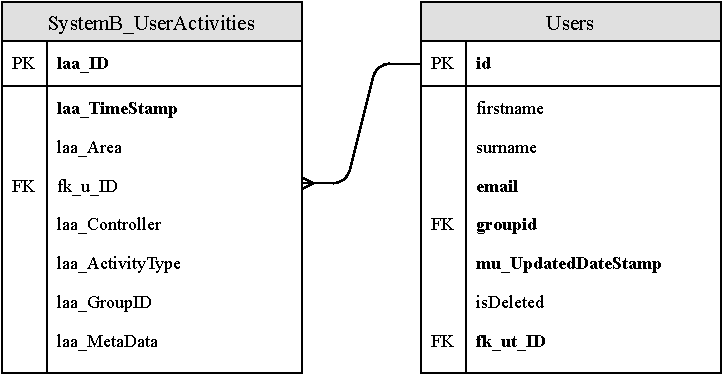
\includegraphics[width=0.99\textwidth]{Chapter2/SystemB_ERD_Basic/SystemB_ERD_Basic.pdf}
	\caption[ERD of user activities]
	{\textit{ERD of the user activities}}\label{fig:ch2_erdOfEventLogs}
\end{figure}

In \Cref{fig:ch2_erdOfEventLogs} is an ERD diagram that describes the relationship of the table created to store the log attributes with other relevant tables. In the system utilisation analysis, this enables different fields of the other tables to be used to categorise the logs. 

\clearpage

\subsubsection{Server side logging point}\label{sec:ch2_serverSideLoggingpoint}
In \Cref{sec:ch2_loggingPoints} the functional requirements for the logging point need to be fulfilled to create a suitable logging point for a software system to track user-based activities. The \textit{HTTP request} will call a function in the system, subsystem or web page to execute the user's actions, this \textit {request} information can be obtained and parsed onto the logging point.\par The logging attribute can be created as a centralised code segment that all the software system's components can execute before executing the targeted software system in Web applications such as:

\begin{itemize}
	\item In most software frameworks the \textit{HTTP request} data can be extracted from the in-build \textit{HTTP request} models to obtain the custom request headers set on the client side. There should be at least a common global location in the software where a single logging point can be called for every \textit{HTTP} function to execute the logging point first before continuing with the rest of the main targeted function. The rest of the log attributes can also be obtained during the execution run time:
	\begin{itemize}
		\item \textbf{Absolute URI path:} The string containing the absolute URI path of the currently active system, subsystem or web page. 
		\item \textbf{Absolute request URL:} The requested URL contains the targeted system, subsystem or web page name and function that the request needs to be executed. 
		\item \textbf{Action parameters:} During the run time some of the parameters which are the request parameters sent with the \textit{HTTP request} from the client device can be obtained.
	\end{itemize}
	\item In other older Web applications that is created with programming languages such as \texttt{PHP} a more direct approach needs to be taken when accessing the request data. In this case, using multiple logging points that call the logging points' main code segment to capture the attributes and store the log in a database. The parameters may need to be extracted before parsing them to the main logging point code segment.
\end{itemize}

As long as the logging attributes and the \textit{HTTP request} headers are obtainable, the logging mechanism can be created on the server side to extract the data and process it. The activity type can be resolved by the defined cases e.g. if the request calls the \texttt{Index} function of the system, subsystem or web page, it can be identified as the Web page accessed user activity type (\ref{fr:uatType1}) of \Cref{tbl:ch2_userActivityTypes}.\par If the user-based event is using the system, subsystem or web page or functions that modify the session, it can be classified as session changed event (\ref{fr:uatType3}) and the rest of the user-based activity events need to be tested afterwards if they meet certain criteria defined for the general activity types. If it fails all three types of classification the event is likely, not user-generated or comes from \textit{HTTP request} that was executed after the initial first request. In such cases, the last HTML element id that triggered the event should not be listed as a clicked element in JavaScript.

\subsubsection{Server side log parsing}
In \Cref{fig:ch2_loggingParse} is the server-side log parsing of the obtained possible user-based activity events for the software system.

\clearpage

\begin{figure}[!htb]
	\centering
	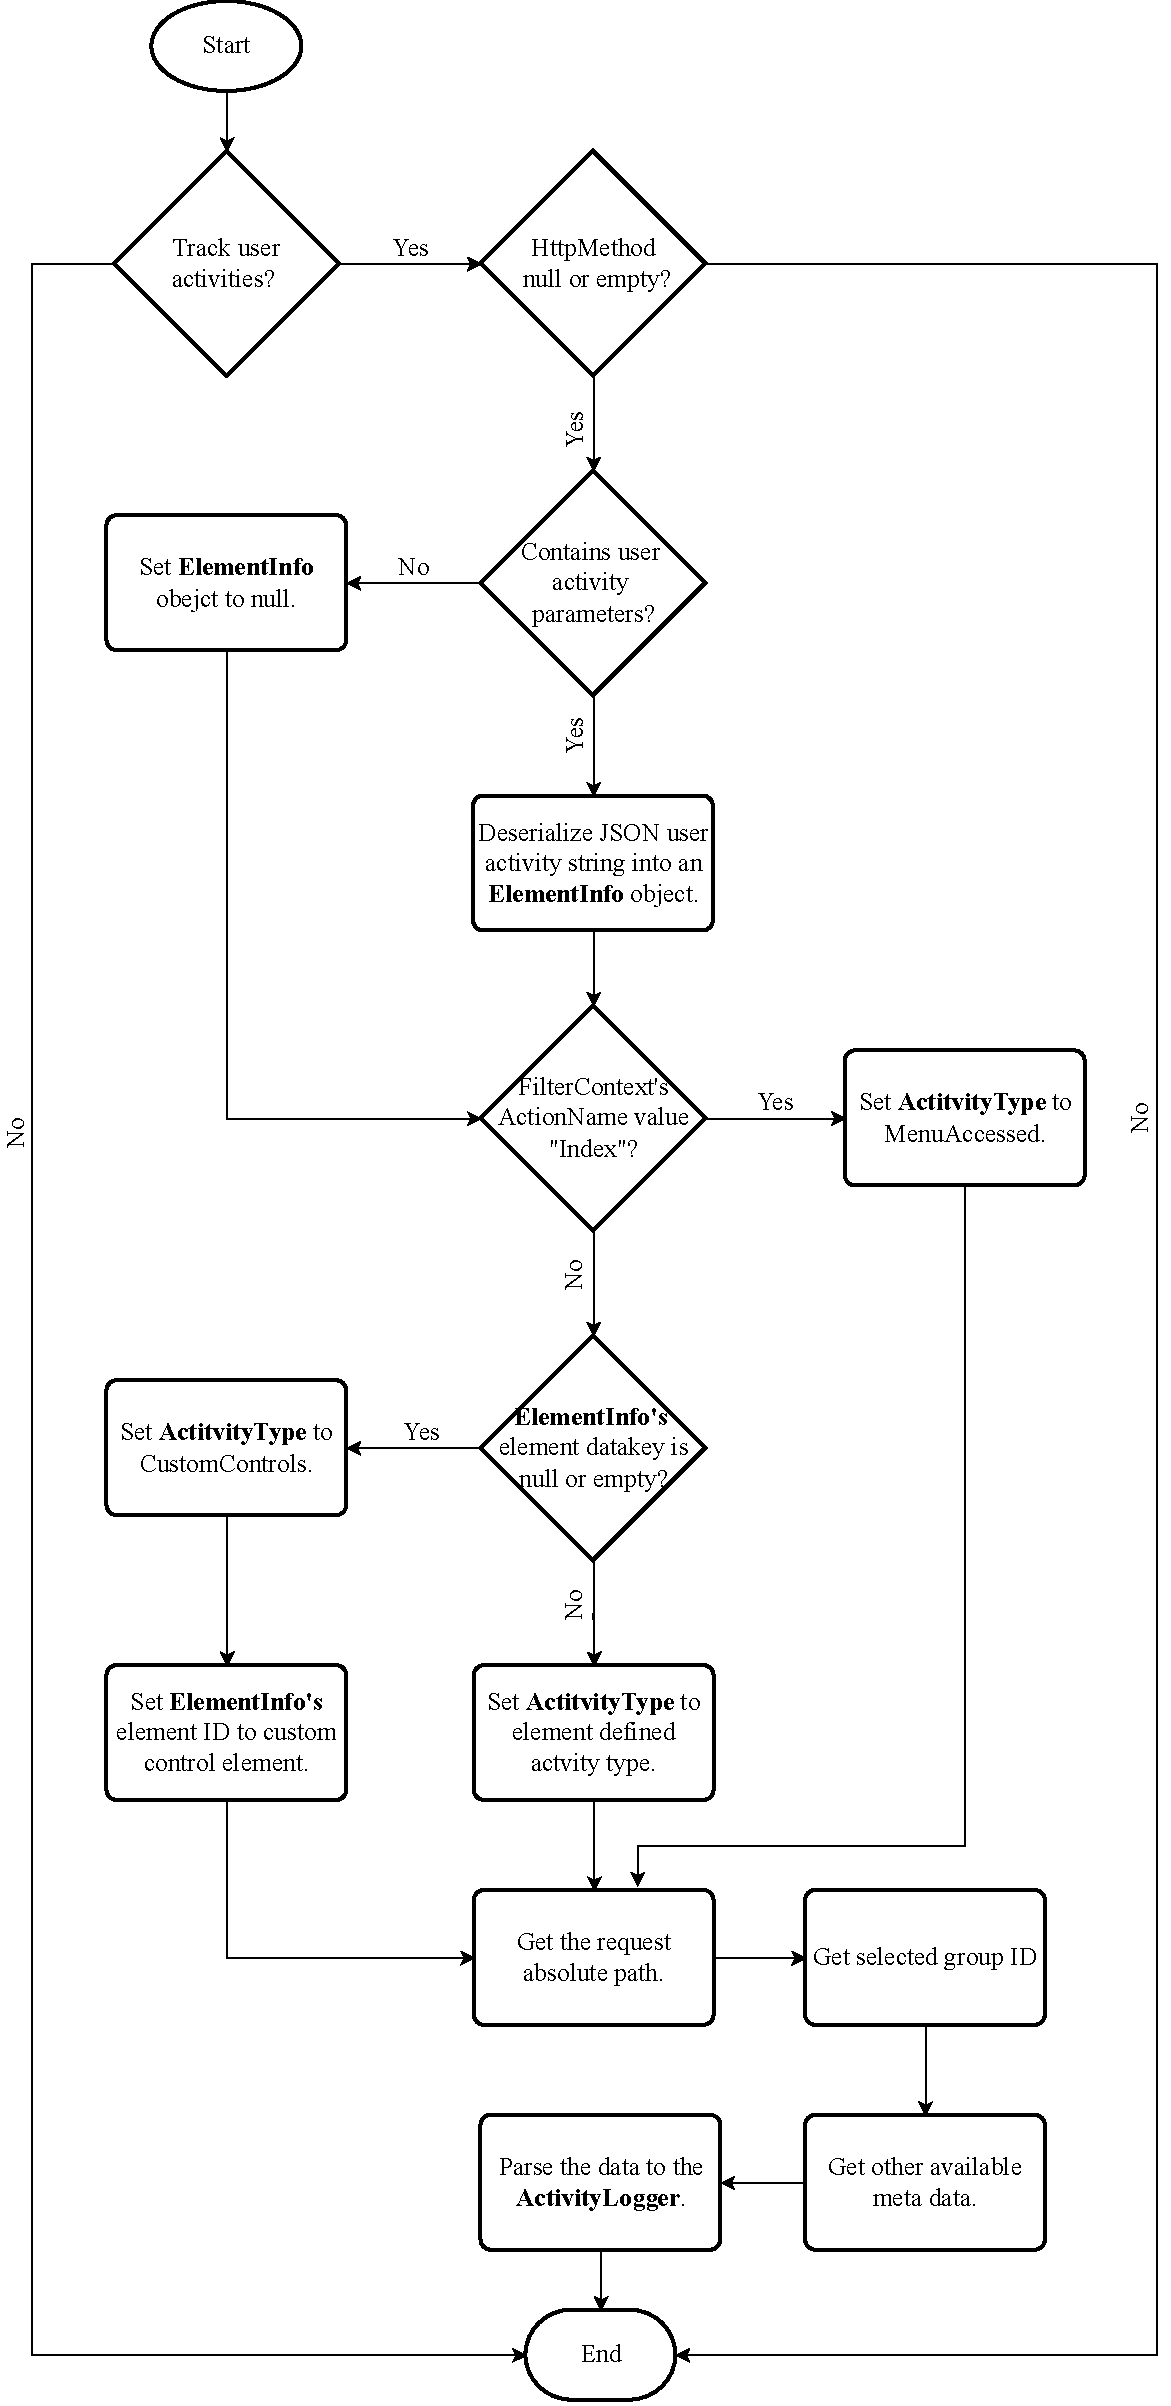
\includegraphics[width=0.7\textwidth]{Chapter2/SystemB_FilterContext/SystemB_FilterContext.pdf}
	\caption[Server side log parsing flow diagram]
	{\textit{Server side log parsing flow diagram}}\label{fig:ch2_loggingParse}
\end{figure}

\clearpage

The defined globally set logging point will start the user-based activity process before the targeted process is executed in \Cref{fig:ch2_loggingParse}. At this stage, if anything goes wrong with the logging at during the execution of this filter, it should be abandoned and let the software system continue to ensure that it doesn't interfere with the software system's operations (\ref{fr:lpa4} of \Cref{tbl:ch2_loggingPointRequirement}).\par In the case of the request method \texttt{NULL} or empty due to errors such as incorrect parameter types for the targeted procedure in the controller, the logging point should stop attempting to log the user-based log. The issue would most likely appear as a run time error and any user-based activity logging procedures will also fail due to incomplete data or cause the logs to be not complete and consistent (\ref{fr:lpa3} of \Cref{tbl:ch2_loggingPointRequirement}).\par If the captured user-activity log contains any parameters it should be checked for any session-related parameters or any other potential user data that should be removed from the metadata to prevent any personal information from being accessed by not the owner of the user account. If it doesn't contain any request parameters the \texttt{ElementInfo} should be set to \texttt{NULL}.\par In \Cref{fig:Ch2_ElementInfo} is the \texttt{JSON} data of the \texttt{ElementInfo}. 

\begin{lstlisting}[style=json, caption={\textit{Element properties JSON}}, label={fig:Ch2_ElementInfo}] 
	{ "ElementTagName" : "button",
		"ElementID" : "submitButton",
		"ElementDataKey": "submit-control"		
	}
\end{lstlisting}

Each of the properties in \Cref{fig:Ch2_ElementInfo} which consist of:

\begin{itemize}
	\item \texttt{ElementTagName}, is the HTML element's tag name which is one of the defined accepted tag names such as \texttt{button}, \texttt{label} and \texttt{td} etc.,
	\item \texttt{ElementID}, identification of the element if it has been assigned to the element and can be obtained on the client side,
	\item \texttt{ElementDataKey}, additional captured data attributes that expand on the identity of the element if it is a custom-made HTML element control. Some software systems may have other custom-created HTML elements which also can trigger a user-based activity. It can be other miscellaneous elements such as a \texttt{label} which are not normal input controls.
\end{itemize}



If the \texttt{request header} contains the \texttt{Index} keyword which is the first procedure that needs to be executed for a Web page being accessed, the activity can be classified as accessing a system, subsystem or web page. This activity type is the first user activity type at this point of the log parsing before it is processed again to another user activity type. \par If it is not the \texttt{Index} the process will continue to the next operation which checks if the \texttt{ElementInfo}'s \texttt{ElementDataKey} is either a null or empty value. If there is any data available the activity type can be set to the custom control defined activity type or just custom control to represent all these custom-made elements. The \texttt{ElementID} is set to the custom control element or the defined custom control's identification. \par If the \texttt{ElementInfo}'s \texttt{ElementDataKey} is null or an empty value the user activity type is set to the element's defined activity type. After the activity type is resolved the request origin of the user-based activity is obtained by getting the request's absolute path.\par After the request origin has been obtained, other relevant session information such as the group that represents a certain entity data can be obtained as well as the user's identification and other relevant metadata that is available at this stage to complete the log attributes that needs to captured from \Cref{tbl:ch2_keyLoggingAttributes} to complete the user-based activity log.\par The data is parsed to the activity logger that will write the log into a database if the log was successfully obtained. This will end the logging process until a new user-based event log is ready to be processed and stored in the database.

\subsection{Client functional requirements interaction}
\par In \Cref{fig:ch2_user_based_actvity_classification} is the complete process of the user interacting with the user interface to trigger a user-based activity event to be logged later for the client's functional requirements. It starts with the user interacting with the user interface. The default activity type is set to general activity (\ref{fr:uatType3}) until it is further processed later in the logging mechanism.\par If the activity has any additional metadata such as other request parameters, it will also be logged by adding searching for it in the completion of the \textit{HTTP request} operation. The other metadata can also be captured in this stage from the client side like the element that the user clicked to initiate the event. The captured metadata is placed in a custom request header afterwards, and the \textit{HTTP request} continues its normal operations and sends the data back to the server.

\begin{figure}[!htb] % An h :here, t: top, b: bottom.
	\centering % cent the figure
	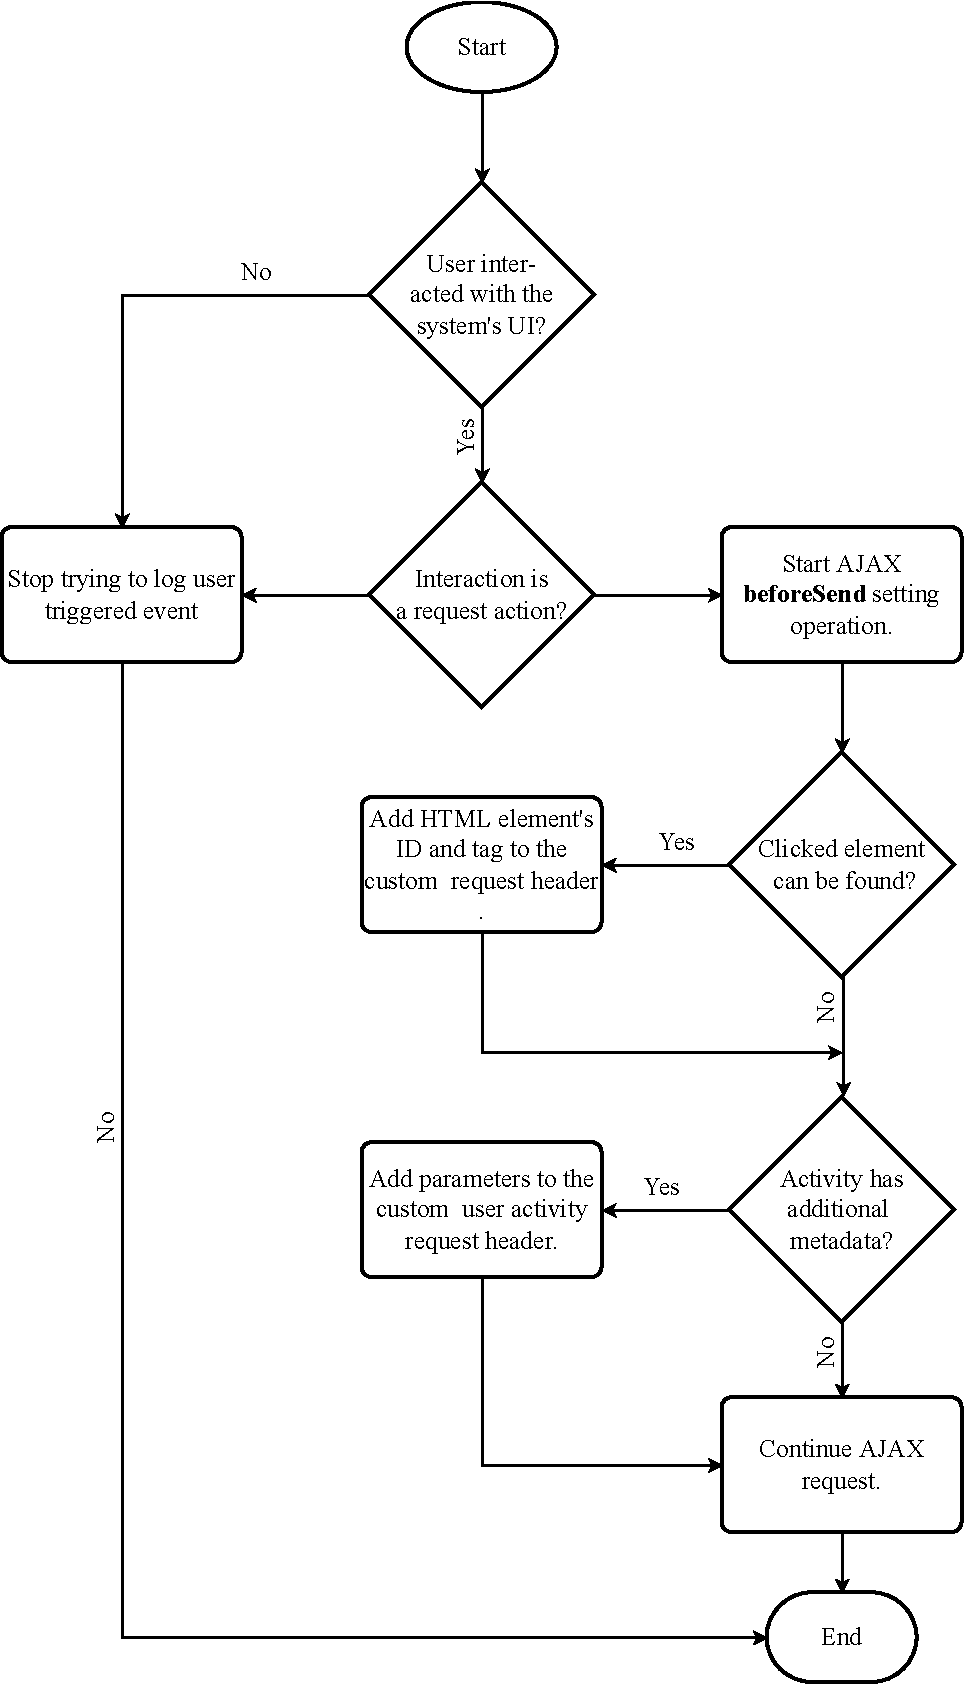
\includegraphics[width=0.75\textwidth]{Chapter2/client_functional_requirement_flow_diagram/client_functional_requirement_flow_diagram.pdf}
	\caption[User-based activity log classification flow diagram]
	{\textit{User-based activity log classification flow diagram}}\label{fig:ch2_user_based_actvity_classification}
\end{figure}

\clearpage

\section{Log analysis}\label{ch2:sec_system_utilisation_analysis}
The log analysis system design will be defined in this section. There are no restrictions on what log analysis tools developers can use but they need to use or implement one that will able to do the log analysis. This section also defines all the sub-functional requirements for the creation or use of log analysis tools (\ref{fr:logAnalysis}) and maintenance prioritising (\ref{fr:maintenancePrioritising}).

\subsection{Create or use log analysis tools}
The log analysis (\ref{fr:logAnalysis}) makes use of either third-party analytical tools or custom-created software log analysis implementations. Developers should use the implementation that will fulfil their log analysis needs. In \Cref{tbl:ch2_logAnalysis} is the log analysis functional requirements (\ref{fr:logAnalysis}).

\setcounter{phase}{3}
\setcounter{subphase}{0}
\begin{table}[!htb]
	\centering
	\caption[Log analysis functional requirements (\ref{fr:logAnalysis})]
	{\textit{Log analysis functional requirements (\ref{fr:logAnalysis})}}
	\label{tbl:ch2_logAnalysis}
	\begin{tabularx}{\textwidth}{|l|l|X|}
		\hline \textbf{Requirement ID} & \textbf{Name} & \textbf{Description} \\
		\hline \subphase{fr:logQuality} & Log quality & \RaggedRight Log quality ensures that the obtained logs are usable for the log analysis. Any incomplete logs should be either fixed in the log analysis implementation or the logging mechanism should be adjusted to get the complete logs. \\
		\hline \subphase{fr:logAnalysisTool} & Log analysis tool requirement & \RaggedRight Certain basic requirements are needed for the log analysis tool to implement a log analysis. \\
		\hline
	\end{tabularx}
\end{table}

\subsubsection{Log quality}
Log quality has been identified in \Cref{sec:ch1_loggingQuality} should be important when implementing a logging mechanism to do log analysis. The log quality (\ref{fr:logQuality}) will both impact the logging mechanism's performance and the accuracy and completeness of the log quality.  In \Cref{tbl:ch2_utilisation_requirements} are the functional requirements for the log quality (\ref{fr:logQuality}).

\setcounter{phase}{3}
\setcounter{subphase}{1}
\begin{table}[!htb]
	\centering
	\small
	\caption[Log quality functional requirements (\ref{fr:logQuality})]
	{\textit{Log quality functional requirements (\ref{fr:logQuality})}}
	\label{tbl:ch2_utilisation_requirements}
	\begin{tabularx}{\textwidth}{|l|l|X|}
		\hline \textbf{Requirement ID} & \textbf{Requirement name} & \textbf{Description} \\
		\hline \subsubphase{fr:ur1} & Log availability & \RaggedRight The user-based logs should be available for any defined period the logging mechanism was actively capturing the user-based events. \\
		\hline \subsubphase{fr:ur2} & Log completeness & \RaggedRight The user-based logs should be complete and there should be minimal corrections made post-logging during the log extraction process (\ref{fr:ur3}) and visualisation presentation. \\
		\hline \subsubphase{fr:ur3} & Log extraction & \RaggedRight The user-based logs are extracted from the database and imported into a visualisation presentation for the user-based activity logs. \\
		\hline
	\end{tabularx}
\end{table}

The log availability (\ref{fr:ur1}) and completeness (\ref{fr:ur2}) functional requirements can be achieved all the functional requirements of the user-based activity log in \Cref{sec:ch2_requirementsOfUAT} are accomplished with minimal processing of the raw logs afterwards. There will be always changes made to the system that can impact which possible user-based events are considered to be logged.\par Log extraction refers to the methods used to obtain the logs from the database with any other relevant data that can be used in the visualisation presentation (\ref{fr:ur4}). The raw logs will need to make use of the foreign references to other tables in the database to provide more detail about the user-based event log as in \Cref{fig:ch2_erdOfEventLogs}.

\subsubsection{Log analysis tool}
The log analysis tool functional requirement (\ref{fr:logAnalysisTool}) is to ensure whether a third-party or custom implementation is done. Will be able to fulfil some basic log analysis requirements defined in \Cref{tbl:ch2_logAnalysisToolFR}.

\stepcounter{subphase}
\begin{table}[!htb]
	\centering
	\small
	\caption[Log analysis tool functional requirements (\ref{fr:logAnalysisTool})]
	{\textit{Log analysis tool functional requirements (\ref{fr:logAnalysisTool})}}
	\label{tbl:ch2_logAnalysisToolFR}
	\begin{tabularx}{\textwidth}{|l|l|X|}
		\hline \textbf{Requirement ID} & \textbf{Requirement name} & \textbf{Description} \\
		\hline \subsubphase{fr:ur4} & Log visual presentation & The visual presentation of the extracted logs should be shown to the user that will make use of the activity logs in a custom visual system or make use of other third-party tools. This will impact how the logs will be extracted (\ref{fr:ur4}) from the database as third-party systems may make use of an API to get the logs from the database. \\
		\hline \subsubphase{fr:ur5} & Log comparison & \RaggedRight By Using the F/R 3.2 the utilisation between different log attributes that are used as the defined criteria. This will be to group and compare different types of users, subsystems and activity types against each other etc.\\
		\hline \subsubphase{fr:ur6} & \RaggedRight Maintenance suggestion & Maintenance suggestions can be made from the system utilisation reports by prioritising maintenance or decommissioning software systems. This can be data or visual representations of the log comparison (\ref{fr:ur5}) using the log visual presentation systems (\ref{fr:ur6}) or creating a summary report from the visual presentation that contains the maintenance suggestions. \\
		\hline
	\end{tabularx}
\end{table}

Each of these functional requirements ensures that the system utilisation analysis will be achieved for the created logging mechanism in \Cref{sec:ch2_loggingMechanism}. The main user interface of the system utilisation analysis will consist of the presentation of the user-based activities (\ref{fr:ur4}). This system will either be a custom-created system to display these logs or third-party software such as Microsoft's business intelligence platform, PowerBI. \par Using the third-party tools has advantages over creating custom software for the visual presentation (\ref{fr:ur4}):

\begin{itemize}
	\item \RaggedRight Third-party BI platforms provide all necessary analytical functionality, making it easy to create visual representations with minimal programming.
	\item \RaggedRight The advanced tools in these platforms offer many ways to visualize user-based activity logs for log comparison (\ref{fr:ur5}).
	\item \RaggedRight Maintenance and editing of these representations are usually trouble-free, with ample support and guides available for developers to make updates to custom visual presentations.
	\end{itemize}

These third-party tools do indeed have some other drawbacks such as:

\begin{itemize}
	\item \RaggedRight Third-party BI platforms are likely to require a subscription, which can be costly for a company license.
	\item \RaggedRight Additional courses may be necessary to fully utilize the capabilities of these platforms.
	\item \RaggedRight Additional functionality, may be required for log extraction (\ref{fr:ur3}) to import data into the platform.
	\end{itemize}

With the drawbacks listed above the third-party business intelligence platforms is the better visual presentation tools for the system utilisation analysis if it is available for use than creating and managing a custom visualisation platform.

\subsection{Maintenance prioritisation}\label{sec:ch2_utilisationImprovements}
Maintenance prioritisation is done from the log analysis. The maintenance prioritising functional requirements (\ref{fr:maintenancePrioritising}) are shown in \Cref{tbl:ch2_maintenancePriortising}.

\setcounter{phase}{4}
\setcounter{subphase}{0}
\begin{table}[!htb]
	\centering
	\caption[Maintenance prioritising functional requirements (\ref{fr:maintenancePrioritising})]
	{\textit{Maintenance prioritising functional requirements (\ref{fr:maintenancePrioritising})}}
	\label{tbl:ch2_maintenancePriortising}
	\begin{tabularx}{\textwidth}{|l|l|X|}
		\hline \textbf{Requirement ID} & \textbf{Name} & \textbf{Description} \\
		\hline \subphase{fr:systemUtiReq} & System utilisation analysis categories & \RaggedRight The system utilisation analysis categories is needed to complete the log analysis. These categories will provide the needed data to make recommendations on how to prioritise software maintenance by using these log analysis metrics.\\
		\hline \subphase{fr:maintenanceFactor} & Maintenance factor & \RaggedRight The maintenance factor measures the amount of maintenance required for a given software system. This will be used to prioritise the software maintenance efforts of the software developers using a scoring system. \\
		\hline
	\end{tabularx}
\end{table}

The system utilisation analysis aims to provide maintenance recommendations to the developers to improve their maintenance efforts by:

\begin{itemize}
	\item Prioritising the maintenance efforts on more frequently used systems.
	\item Decommission unused systems. The user-based activities provide a quantitative reason why certain systems can be decommissioned due to inactivity from the users.
\end{itemize}

This can be achieved by implementing a maintenance prioritising using \Cref{eq:ch2_maintenanceFactorSimplified}:

\begin{equation}
	\label{eq:ch2_maintenanceFactorSimplified}
	M_{PF} = A_{N} \times P_{N}
\end{equation}

where:

\begin{itemize}
	\item $M_{PF}$ is the maintenance priority factor,
	\item $A_{N}$ is the normalised activity for the total logs obtained per subsystem,
	\item $P_{N}$ is the normalised priority factor for the subsystem.
\end{itemize}

The normalised user activities per subsystem are described by \Cref{eq:ch2_eventNormalised}:

\begin{equation}
	\label{eq:ch2_eventNormalised}
	A_{N} = \frac{A_X - A_{Min}}{A_{Max} - A_{Min}},
\end{equation}

where:

\begin{itemize}
	\item $A_X$ is the total obtained user activities for the specified subsystem
	\item $A_{Min}$ is the total minimum user activities for a subsystem,
	\item $A_{Max}$ is the total maximum user activities for a subsystem.
\end{itemize}

The normalised priority factor $P_N$ is described in \Cref{eq:ch2_priorityNormalised}:

\begin{equation}
	\label{eq:ch2_priorityNormalised}
	P_{N} = \frac{P_X - P_{Min}}{P_{Max} - P_{Min}},
\end{equation}

\begin{itemize}
	\item $P_X$ is the total obtained users that have access to the subsystem,
	\item $P_{Min}$ is the total minimum number of users that have access to any subsystem,
	\item $P_{Max}$ is the total maximum number of users that have access to any subsystem.
\end{itemize}

A normalised value for the priority is used as there isn't a predefined way how to describe the importance of any subsystem.

\clearpage

\subsubsection{System utilisation analysis categories}
The system utilisation analysis categories functional requirements (\ref{fr:systemUtiReq}) is used to categorise the log data for the maintenance prioritising metrics. In \Cref{tbl:ch2_utilisationCategories} is the system utilisation analysis categories functional requirements (\ref{fr:systemUtiReq}).

\begin{table}[!htb]
	\centering
	\caption[System utilisation analysis categories functional requirements (\ref{fr:systemUtiReq})]
	{\textit{System utilisation analysis categories functional requirements (\ref{fr:systemUtiReq})}}
	\label{tbl:ch2_utilisationCategories}
	\begin{xltabular}{\textwidth}{|l|l|X|}
		\hline \textbf{Requirement ID} & \textbf{Requirement name} & \textbf{Description} \\
		\hline \subsubphase{fr:utCategories1} & Users & The users of the software systems can be put in different categories based on who uses the software. This can be both the customer users or the employees using the software. Using the activities of the customer users will provide the data on which systems the development team needs to put their resources into. \\
		\hline \subsubphase{fr:utCategories2} & User activity types & The user activity types in \Cref{tbl:ch2_userActivityTypes} can be used as a category to compare different user-based activity types with each other and use a sub-category for categories such as the different users that can use the system (\ref{fr:utCategories1}). \\
		\hline \subsubphase{fr:utCategories3} & Systems or subsystems & The request origin (\ref{fr:lpa5}) of the user-based activities can be categorised to compare different subsystems and controllers to each other.\\
		\hline \subsubphase{fr:utCategories4} & Miscellaneous categories & This user-based activity category type will make use of the metadata attribute (\ref{fr:lpa7}) of \Cref{tbl:ch2_keyLoggingAttributes}. The other fields which are not set as main categories can be also placed in this category as they can take multiple forms.\\
		\hline
	\end{xltabular}
\end{table}

The categories in \Cref{tbl:ch2_utilisationCategories} enable the log data to be placed in different categories to compare them to each other. A software maintenance prioritising model can be made with the comparisons of these categories.

\section{Conclusion}
In \Cref{sec:ch2_loggingMechanism} are the defined functional requirements for a logging mechanism for the system utilisation analysis in \Cref{ch2:sec_system_utilisation_analysis}. The user activity types defined in \Cref{sec:ch2_userActivityTypes} are the base of what log attributes need to be logged to create a user-based log.\par The logging points capture logs and send them to the server's logging point where it is processed and stored in writing in a database.\par The logs are extracted into a visual presentation which enables the maintenance improvement suggestions based on the utilisation analysis in \Cref{ch2:sec_system_utilisation_analysis}.